\documentclass{article}
\usepackage{graphicx} % Required for inserting images
\usepackage[margin=1in]{geometry}
\usepackage{url}
\usepackage{hyperref}

\usepackage{float}
\usepackage{amsmath}
\usepackage{amssymb}

\usepackage{pdfpages}

\usepackage[calc]{datetime2}
\usepackage{pgfgantt}
\usepackage{datenumber}

\usepackage{pdflscape}

\title{CS310 Progress Report: Evaluating the Performance of Blink Detection on DeepFakes Injected With Adversarial Noise}
\author{Joel Coulon, 2204489}
\date{}

\begin{document}

\maketitle

\section{Project Introduction}

A DeepFake refers to when a video of an individual is digitally altered or created by an Artificial Intelligence (AI). These are often generated using Generative Adversarial Network models (GANs) and are trained via two competing models: one attempting to generate a realistic image, the other trying to detect the inaccuracies. These two then train each other until the generator model can create videos that are deemed realistic by the detector. A DeepFake is born.\\

Initially, these models were fairly easy to detect, even for humans (see Figure \ref{fig:earlyexample}). Various features, such as temporal inconsistencies, facial feature irregularities, and inconsistencies in lighting were all tell-tale signs of a DeepFaked image. However, over time, GANs have developed, resulting in DeepFakes now being almost impossible to tell apart from genuine videos by humans.

\begin{figure}[H]
    \centering
    \fbox{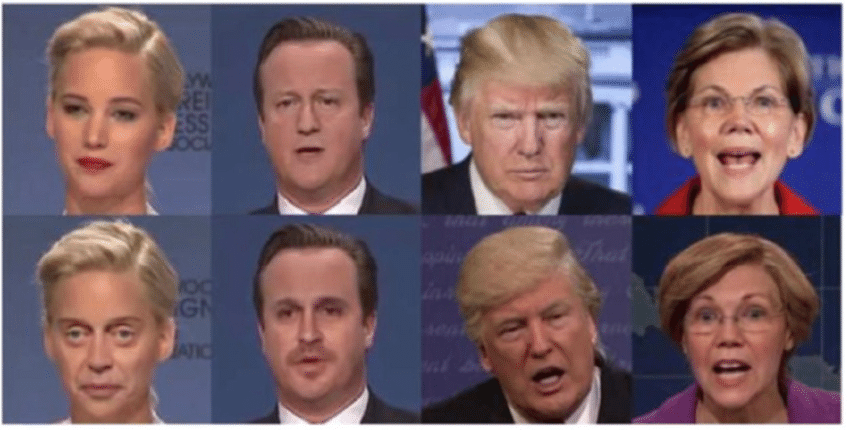
\includegraphics[width=0.5\linewidth]{images/Examples-of-original-and-deepfake-videos.png}}
    \caption{An early of example of DeepFakes with original images on the top, faked images on the bottom\cite{earlydeepfakeimage}}
    \label{fig:earlyexample}
\end{figure}

Due to their difficulty in being accurately identified by humans, DeepFakes soon became a popular way to spread misinformation by faking an individual's likeness. For example, DeepFakes were used by a variety of sources to promote political parties in the 2021 Lebanese elections\cite{misinformation}. The other primary use of DeepFakes is pornography with an estimated 98\% of DeepFakes being porn\cite{pornography}, including the first main-stream DeepFake of actress Gal Gadot in 2017\cite{misinformation}.\\

Ever since the creation of DeepFakes, there have been efforts to detect them. Original DeepFake detection methods relied on pixel analysis and visual artifacts present in early DeepFakes\cite{yu2021survey}. However, through a combination of improvement in generation techniques and adversarial noise attacks\cite{huang2020fakeretouch}\cite{pertubations}, these original methods are proving increasingly ineffective.\\

One method proposed to tackle modern DeepFakes is blink detection. Blinking is a subconscious act for humans and falls into predictable patterns. DeepFakes are notoriously bad at simulating blinking, either by not blinking at all or in unnatural intervals. Thus various methods have been used to leverage blinking inconsistencies to detect DeepFakes with a high degree of accuracy\cite{blinking-pattern}.\\

The resilience of blink detection to adversarial noise has yet to be studied. It seems likely that, due to this method relying on the identification of features rather than individual pixels, adversarial noise would have little effect the detection of DeepFakes. This project aims to verify whether this assumption is true or not.

\section{Literature Review} \label{sec:literature-review}

This project combines two thoroughly-research topics: blink-based DeepFake detection and adversarial noise injection, which have had extensive research on both of them. The following is a summary on the key ideas and techniques.

\subsection{Blink Detection}
\subsubsection{DeepVision}

DeepVision\cite{blinking-pattern} is a model that takes into account the time, activity, gender and age of the individual in a video to determine whether a video is DeepFaked or not by comparing their blink patterns to a database of known ``good" blinking patterns.\\

The pre-processing stage of the model involves categorising the video based on 4 landmarks. The landmarks are: gender, age (in 6 sub-categories varying from \textless 20 to 65+), activity (dynamic or static), and time (am/pm). The frequency of a human varies based on all these features\cite{varying-blink}, and therefore they believe all of these factors need to be considered for accurate detection.\\

Two algorithms are used to detect a blink. The first is an algorithm called Fast-HyperFace\cite{ranjan2017hyperface} which is used to detect the landmarks of the face, pose, and gender of the individual in a video. The eye locations are then extracted to run the second model: Eye-Aspect Ratio (EAR). EAR uses 6 points to calculate the absolute area of the horizontal versus the vertical axis to determine if a blink has occurred\cite{EAR}.
\begin{equation}
    EAR=\frac{||p_2-p_6||+||p_3-p_5||}{2||p_1-p_4||}
\end{equation}
The average of the left eye (EAR\textsubscript{l}) and the right (EAR\textsubscript{r}) can then be taken to get the mean eye ratio (EAR\textsubscript{i})
\begin{equation}
    EAR_i = \frac{EAR_l + EAR_r}{2}
\end{equation}
\begin{figure}[H]
    \centering
    \fbox{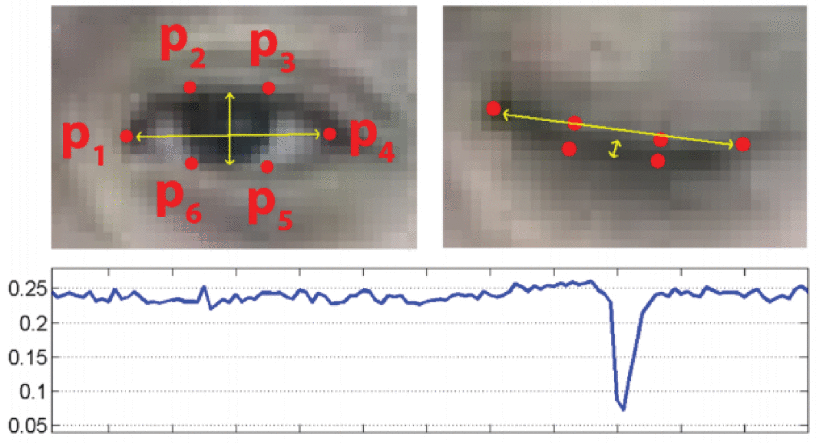
\includegraphics[width=0.5\linewidth]{images/EAR.png}}
    \caption{The EAR algorithm at work with eye landmarks $p_{1-6}$ labelled and a graph representing EAR (y-axis) over time (x-axis)}
    \label{fig:EAR}
\end{figure}

A blink is when EAR\textsubscript{i} drops below a certain threshold for multiple consecutive frames. Data such as when the blink occurred in time, the period of blink, and frequency are all features determined by the EAR with respect to time and can be used by future detection methods.\\

This data is then compared with data from a pre-existing database of valid blinks derived from the Eye Blinking Prediction dataset from Kaggle\cite{eyeblinkprediction}. The factors mentioned above are all compared to see how similar they are to valid blinks in authentic videos. If they within a certain threshold, the video is deemed real. The paper does not mention this threshold.\\

DeepVision achieves an overall accuracy of 87.5\%\cite{blinking-pattern}.

\subsubsection{Ictu Oculi}

Ictu Oculi is a secondary method for blink detection. Rather than relying on an existing database for comparison, it uses a trained neural network\cite{ictuoculi}.\\

An initial pre-processing step is done to identify the facial landmarks of the image and distort and crop it so that the face is: in the centre of the image; rotated such that the eyes form a horizontal line; and scaled to a similar size across the duration of the video.\\

Once pre-processing is complete, the cropped video is sent to a Long-term Recurrent Convolution Neural Network (LRCN) to determine the state of the eyes. This is a three-stage neural network as shown in Figure \ref{fig:LRCN}. 

\begin{figure}[H]
    \centering
    \fbox{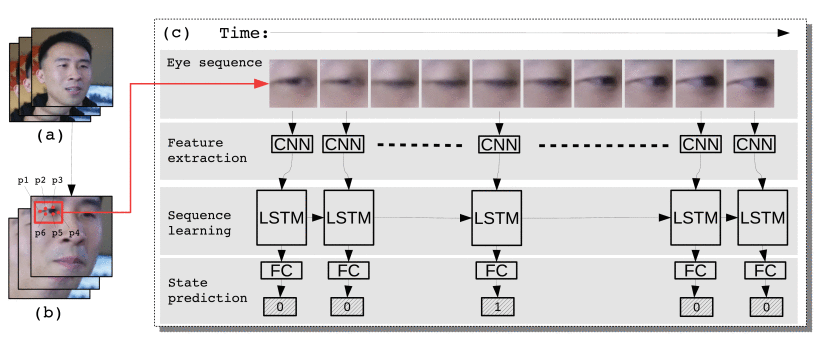
\includegraphics[width=0.75\linewidth]{images/LRCN.png}}
    \caption{Overview of the LRCN method. (a) is the original sequence. (b) is the sequence after face alignment. The eye region of each frame is cropped based on eye landmarks $p_1-6$ in (b) and pass it to (c) LRCN, which consists of three parts: feature extraction, sequence learning and state prediction\cite{ictuoculi}}
    \label{fig:LRCN}
\end{figure}

The first part is a typical Convolution Neural Network (CNN) used to extract the discriminative features from the eye region. The next stage is to use a Recursive Neural Network with Long Short Term cells (LSTM-RNN) to guess the state of the eye with $0$ equating to open, and $1$ being closed. To do this it uses the following functions:

\begin{equation}
\begin{array}{l}
    f_t = \sigma \left( W_{fh} h_{t-1} + W_{fx} x_t + b _f \right) \\
    i_t = \sigma \left( W_{ih} h_{t-1} + W_{ix} x_t + b_i \right) \\
    g_t = \tanh \left( W_{ch} h_{t-1} + W_{cx} x_t + b_c \right) \\
    C_t = f_t \odot C_{t-1} + i_t \odot g_t \\
    o_t = \sigma \left( W_{oh} h_{t-1} + W_{ox} x_t + b_o \right) \\
    h_t = o_t \odot \tanh \left( C_t \right)
\end{array}
\end{equation}

$\sigma$ is the sigmoid function, $f_t$ is forget gate to control what previous memories will be discard, it is input gate to selectively pass the current input, which is manipulated by $g_t$. $o_t$ is output gate to control how much memory will be transferred into hidden state $h_t$. Memory cell $C_t$ is combined by previous memory cell $C_{t-1}$ controlled by $f_t$ and manipulated input $g_t$ controlled by $i_t$. $b_{var}$ is a bias designed to add weight to a specific feature. 256 hidden units are used in the LSTM cell, which is the dimension of LSTM output $z_t$\cite{ictuoculi}. A diagram of such a cell is shown in Figure \ref{fig:LSTM}.

\begin{figure}[H]
    \centering
    \fbox{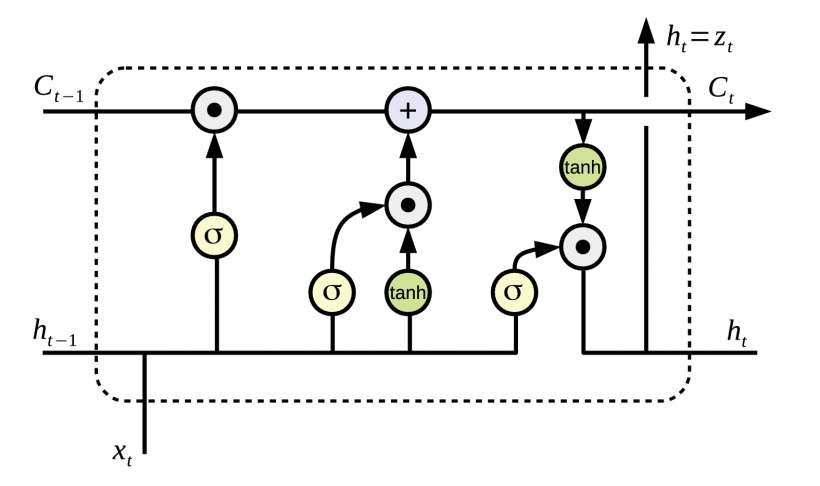
\includegraphics[width=0.5\linewidth]{images/LSTN.png}}
    \caption{A diagram of LSTM structure\cite{ictuoculi}}
    \label{fig:LSTM}
\end{figure}

Finally, the output is determines whether or not a blink has occurred, and over what period.\\

As the accuracy of data is reduced from the amount an eye is open to a binary open/close, the simplicity of the validity algorithm needs to be greatly reduced. The algorithm implemented detects the number of blinks in a set period (60 seconds), the average person blinks 34.1 times a minute. A video is deemed fake or real based on how closely the blinking in the video matches this number. This leads to an accuracy of 99\% when tested on a dataset of 32 videos.

\subsubsection{Analysis}

DeepVision's primary advantage is that it is easy to compute and program. Fast-HyperFace is a pre-trained model and therefore is a simple drag-and-drop implementation. Once $p_{1-6}$ are located in a frame, it is a simple calculation to determine the EAR. The following statistical analysis to determine whether blinking is consistent with real videos is also relatively simple and non-computationally intensive as it is a database query. Therefore, any methodology involving DeepVision would be fast to implement and relatively easy to debug. It also benefits from more granularity in eye state data which could enable more complex analysis.\\

The primary downside to DeepVision is the potential obstruction of the eye(s). EAR requires the entire eye to be visible in the frame of a video to identify all of the points. A partial $EAR$ can be calculated with a single eye but the accuracy of this is going to be less than if two eyes were visible. The second disadvantage is the database required to determine whether blinking is consistent with normal blinking. The database requires many labelled examples which would be time-consuming to produce.\\

Ictu Oculi has a much more complex blink-detection system, requiring two separate machine learning models trained to identify if a blink is happening or not. This is more complex and requires pre-processing resulting in longer development and training times. On the other hand, it results in a much more resilient blink detection mechanism as the eye's state can be accurately determined even when partially obscured.\\

The drawback is that the state of the eye is binary open/close, any information relating to the speed of the blink is lost resulting in a very rudimentary system to determine whether a sequence of blinks is a DeepFake or not. Yet, this has little effect on the accuracy of detection.\\

The planned implementation can be found in Section \ref{sec:future-blink}.

\subsection{Adversarial Noise}

It has been demonstrated by various works that the majority of current DeepFake detectors, even state-of-the-art ones, can be fooled by adversarial attacks\cite{juefei2022countering}. Adverserial attacks work by manipulating the image produced by a DeepFake to try and throw off detectors.

\subsubsection{Adversarial Perturbations}

Adversarial Perturbations Fool DeepFake Detectors\cite{pertubations} is a paper that proposes two unique methods to add adversarial noise. The first way is Fast Gradient Sign Method (FGSM).

\begin{equation}
    \mathbf{x}_{adv} = \mathbf{x} + \varepsilon \operatorname{sign} (\nabla _x J( \mathbf{x},\mathbf{y}, \theta ))
\end{equation}

$\mathbf{x}_{adv}$ is the image produced once the adversarial attack has been completed. $\mathbf{x}$ denotes a vector of pixel value to denote the image produced by a GAN. $J$ is the training loss function (one possible example is categorical cross-entropy loss) which takes $\theta$ as the parameters of the model. Finally $\varepsilon$, is a hyperparamter for the magnitude of perturbation per pixel. A high $\varepsilon$ leads to higher chance to disrupt the model but a higher chance the perturbations become visible to humans, it is recommended to keep $\varepsilon$ in the range [0,01, 0.1]. 0.02 was used in the paper\cite{pertubations}.\\

This is a very primitive method to add noise compared to the other methodologies but is sufficient (Figure \ref{fig:fgsm}). The primary difficulty is choosing $J$ as the loss function can greatly influence inhow effective the noise can be. Too aggressive, and the adversarial noise wll be less effective; too weak and the noise may be obvious to humans. In the paper, they use categorical entropy loss.\\

The other method proposed by \cite{pertubations} is the Carlini and Wagner $L_2$ Norm Attack (CWL\textsubscript{2}). The following method is based on the original paper\cite{carlini2017towards} and a PyTorch implementation\cite{cwl2python}. The first aim is to minimise the $L_2$ norm for the adversarial image $\mathbf{x}'$:

\begin{equation}
\label{eq:l2_norm}
    \mathop {\min} \limits_{x'} \left\{ \left\| \mathbf{x}' - \mathbf{x} \right\|_2^2 \right\}
\end{equation}

The other objective is:

\begin{equation}
\label{eq:min_f(x')}
\begin{array}{c} 
    \mathop {\min} \limits_{x'} \left\{ f\left( \mathbf{x}' \right) \right\} \\
    \text{where } f\left( \mathbf{x}' \right) = \max \left( \max_{i \ne y} \left\{ \mathbf{Z} \left( \mathbf{x}' \right)_y - \mathbf{Z} \left( \mathbf{x}' \right)_i \right\}, - \kappa \right)
\end{array}
\end{equation}

Where $\mathbf{Z}(\mathbf{x}')$ is the product of DeepFake detector. $i$ is the index of the current target class and $y$ is the index of the true target class (if no alterations were made). Thus by minimising $f(\mathbf{x}')$, the difference between the incorrect class ($\mathbf{Z}{{\left( {{\mathbf{x}}'} \right)}_i}$) and the correct class (${\mathbf{Z}}{{\left( {{\mathbf{x}}'} \right)}_y}$) is maximised meaning a miss-classification is more likely. $\kappa$ defines a threshold for the maximum difference between the incorrect and correct classes.\\

To ensure a pixel is only altered by a value between 0 and 1:

\begin{equation}
\label{eq:tanh}
    \mathbf{x}' = \frac{1}{2}(\tanh (\omega ) + 1)
\end{equation}

Thus combining \ref{eq:l2_norm}, \ref{eq:min_f(x')}, and \ref{eq:tanh}:

\begin{equation}
\begin{array}{c}
    \omega^\ast = \arg \min_\omega \left\{ \left\| \mathbf{x}' - \mathbf{x} \right\|_2^2 + cf\left( \mathbf{x}' \right) \right\} \\
    \mathbf{x}_{adv} = \frac{1}{2}\left( \tanh \left( \omega^\ast \right) + 1 \right)
\end{array}
\end{equation}

$c$ is a positive parameter designed to weight the two objectives of the CW-L\textsubscript{2} attack. It is typically found via binary search during run time. Determining the hyperparameters takes a long time, however, leads to better results, especially on whitebox testing:

\begin{figure}[H]
    \centering
    \fbox{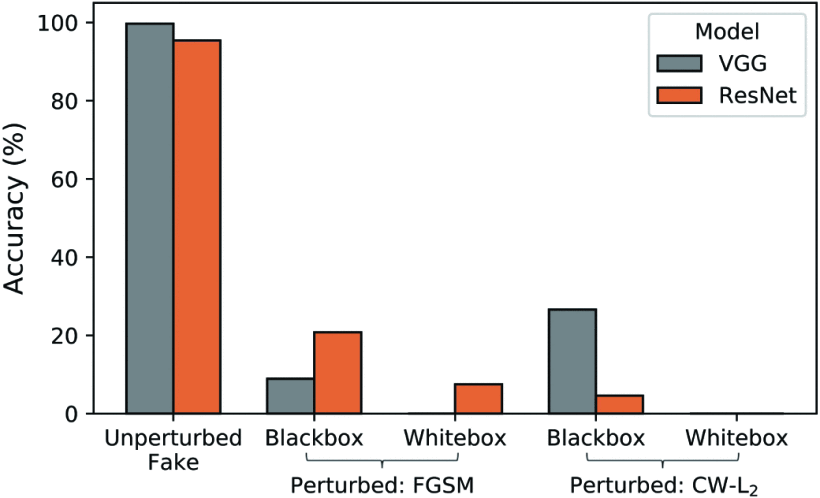
\includegraphics[width=0.5\linewidth]{images/fgsm.png}}
    \caption{Evaluation of FGSM and CW-L\textsubscript{2}}
    \label{fig:fgsm}
\end{figure}

\subsubsection{FakeRetouch}

FakeRetouch is another method of adding noise to an image, using a combination of additive noise and deep image filtering to reduce artifact patterns in both the spacial and frequency domains\cite{huang2020fakeretouch}. The method uses the following equation to produce the doctored image $\hat{\mathbf{I}}$:

\begin{equation}
\begin{array}{c}
    \hat{\mathbf{I}}=\text{DNN}(\mathbf{I})\circledast (\mathbf{I} +\mathbf{A}\odot \mathbf{N}_{\sigma}) \\
    \text{where }\mathbf{A}=\arg \max _{\mathbf{A}}J(D(\mathbf{I}+\mathbf{A}), y) +||\mathbf{A}||_1
\end{array}
\end{equation}

$DNN(\mathbf{I})$ is a UNet-like neural network using kernels of $\mathbf{I}$. When combined with $\circledast$ (pixel-wise filtering), the following method can be done: for the $p$-th pixel in an image $\mathbf{I}$, is altered by the corresponding $p$-th kernel in $\mathbf{K}$ denoted as $\textbf{K}_p \in \mathbb{R}^{K \times K}$ with $k$ being the kernel size \cite{huang2020fakeretouch}. $J(\cdot)$ is a cross-entropy loss function with $y$ as the ground-truth value. $D(\cdot)$ is the DeepFake detection model being targeted. Adding the $L_1$-norm ($||A||_1$) encourages the noise to be sparse to avoid human perception of the noise. Finally, $\odot \mathbf{N}_\sigma$ adds Gaussian Noise filter with standard deviation $\sigma$. \\

The result of this method caused a drop in accuracy of detecting fake images from 88.99\% to 21.64\%. As $DNN(\mathbf{I})$ can be computed offline and then applied to every frame in a dataset, it is overall relatively quick to run.

\subsubsection{Adversarial Patch}

Adversarial Patch confuses DeepFake detectors by adding a specially crafted ``patch" to an image to confuse classifiers\cite{brown2017adversarial}.

\begin{figure}[H]
    \centering
    \fbox{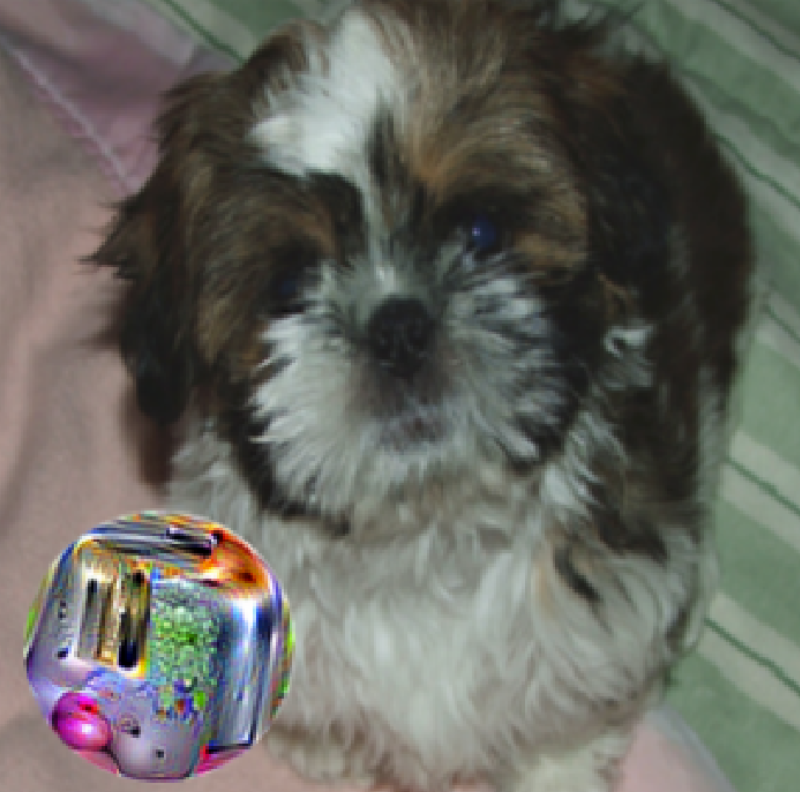
\includegraphics[width=0.25\linewidth]{images/adverserial_patch.png}}
    \caption{An image of a dog with the adversarial patch added in the bottom left to attempt to misclassify the image as a toaster\cite{brown2017adversarial}}
\end{figure}

This methodology will not be used as it is clear to a human that there is something malicious going on with the patch, even if it is not immediately obvious what it would be for.

\subsubsection{Analysis}

FGSM will not be used due to its relative ineffectiveness. As shown in Figure \ref{fig:fgsm}, CW-L\textsubscript{2} is more effective on both black and whitebox attacks.\\

Out of the remaining two methods, FakeRetouch seems to be the quickest and easiest to implement. It also is the quickest to apply as there are no hyperparamters to be fine-tuned\cite{huang2020fakeretouch}. This is a major factor as the model will need to be run on all the videos in the dataset to try, which could be millions, possibly billions of frames, thus efficiency is key. It has slightly worse reported effectiveness than CW-L\textsubscript{2} and FGSM but this is made up for by its speed.\\

Due to its effectiveness, CW-L\textsubscript{2} will also be implemented. This task will be easier as there is already a pre-existing pyTorch implementation\cite{cwl2python}.\\

The planned implementation can be found in Section \ref{sec:future-noise}

\subsection{Datasets}

There is an extensive range of DeepFake datasets due to their potential to produce misinformation and other damaging content. One such example is FaceForensics++\cite{roessler2019faceforensicspp}, a vast (approximately 2TB) dataset of short clips generated through various generation methods. Once you get access, you also get access to Google's \& JigSaw's DeepFake Detection Dataset\cite{DDD_GoogleJigSaw2019} which contains a (slightly smaller) set of videos.\\

Meta has also created a detection dataset\cite{DFDC2020}, made available through Kaggle\cite{kagglemeta}. This dataset contains 124,000 videos created by 8 different DeepFake generators to create a comprehensive dataset.\\

The final dataset being used is FakeAVCeleb\cite{khalid2021fakeavceleb}. It consists of videos of celebrities from five racial backgrounds (Caucasian (American),  Caucasian (European), African, Asian (East), and Asian (South)) intended to ``counter the racial bias issue" present in a lot of modern DeepFake generators and detectors.\\

An analysis on how these datasets will be stored can be found in Section \ref{sec:datasets}

\section{Current Progress}

\subsection{Delay} \label{sec:delay}

Unfortunately, the project is currently delayed by approximately two weeks. This is due to two reasons: courseworks and extent of research required.

\subsubsection{Courseworks}

In the specification, it was stated: ``whilst other modules have their coursework at the same time as this project is happening, with effective time management, there will be no major clash with timings; at least not enough to delay the course of the project significantly." It turns out some of the courseworks were more work than anticipated, most notably the compilers coursework. This led to the project being delayed by roughly two weeks.\\

To remedy this, Wednesday afternoons have been set aside as dedicated time to work on the project. Other times will also be used should there be any free time available. Additionally, next term, I will be taking fewer modules, which will have smaller courseworks, and thus, the workload that is not project-related will be reduced.

\subsubsection{Research Required}

The initial project specification was written assuming that the project would only implement an existing DeepFake detection methodology that only existed as a theoretical proof of concept. The chosen methodology, blink detection, involves two models: one to determine the state of the eyes, and the other to determine whether the sequence produced by the previous model is feasible. Additionally, methods to add adversarial noise to images needed to be researched. Thus the research phase took three weeks rather than the intended two, further setting the project behind.

\subsection{Literature Review}

The majority of progress made on this project has been the literature review as detailed in Section \ref{sec:literature-review}. This involved researching the various aspects of the field and seeing what existing research. For example, for blink detection, comparing DeepVision versus Ictu Oculi.\\

After reviewing the available literature, works were analysed to work out which approach would be most appropriate in this scenario given: time, difficulty, and effectiveness. Once the various methods were evaluated, a proposal for both a proof of concept and the final version were made. This plan will then be implemented in due course as laid out in Section \ref{sec:future-progress}.

\subsection{Datasets} \label{sec:datasets}

DeepFake detection datasets are extensive so there is a difficulty in how they can be stored. The typical maximum allowance for an account on the Department of Computer Science's systems is 500GB (an increase from 25GB)\cite{dcsquota}. The department has been contacted about the viability of storing such a large amount of data (approximately 10TB once images have been updated with a noise mask). Possible solutions are: to use old hard drives and attach them to the existing computer science compute cluster; use the  Scientific Computing Research Technology Platform (SCRTP) clusters which have the appropriate specifications to handle large volumes of data; or to only test partial amounts of each dataset at a time. An account has been created for SCRTP, and access to Avon (SCRTP's HPC cluster) has been requested.\\

To access most of the datasets, a Google form has to be completed to prove that you will only use the dataset for academic purposes. Such forms for all relevant datasets have been completed. As of writing (18th November), permission has been granted to access FaceForensics++, Google's DeepFake Detection Dataset, and FakeAVCeleb. A Kaggle account has yet to be created access to Meta's Deep Fake Detection Challenge Dataset.

\section{Future Progress} \label{sec:future-progress}
\subsection{Proof of Concept}

Over the Christmas holiday, to test if all the research presented previously is valid, a proof of concept of both the blink detection mechanism and adversarial noise injector will be made and tested end to end. These are intended to be quick to develop and test and so will use pre-trained models and existing codebases, such as Google's MediaPipe\cite{mediapipe} and the PyTorch CW-L\textsubscript{2}\cite{cwl2python}. Inctu Oculi's method of detecting the frequency of blinks will be used to determine if a video is genuine or not.

\subsection{Blink Detection} \label{sec:future-blink}

The primary disadvantage of the EAR is that it cannot calculate the state of an eye if any of $p_{1-6}$ is obscured\cite{ictuoculi}. However, various AI models such as Google's MediaPipe\cite{mediapipe} and OpenFace\cite{openface} can detect these features, even when obscured. Hence it is possible to maintain an accurate EAR even when the face is partially obscured in a frame. Therefore, for the blink detection, MediaPipe will be initially used as a proof of concept and then move on to training a novel model from various eye datasets such as Kaggle's eye blinking prediction\cite{eyeblinkprediction}.\\

Having the EAR data allows for more sophisticated methods of blink detection than what was utilised by Ictu Oculi. However, a technique such as the database employed by DeepVision\cite{blinking-pattern} would be too time-consuming to label and store all the data given the amount of time given to this project. Given the large amount of data available: such as the time taken to blink, the period between blinking, and the overall progression of the EAR it may be possible to train a classifier neural network to determine whether or not a sequence of EAR readings over time is a that of a genuine video or a DeepFake. As this has never been done before, further research and experimentation would need to be done.

\subsection{Adversarial Noise} \label{sec:future-noise}

All methods of adversarial noise injection require the model being targeted to be fully developed, therefore this has to be trained after the blink detection model is trained. Once a proof of concept has been verified and the full blink detector is trained, a full version of FakeRetouch and CW-L\textsubscript{2} shall be trained. Noise will then be applied to all clips in the datasets to then be test the reillience of blink detection to such attacks.

\subsection{Noise Reduction}

Diffusion models are a machine learning concept primarily used for computer vision applications (for example noise reduction and image generation)\cite{croitoru2023diffusion}. They are perhaps most famous for their use in image generation models such as Dall-E by OpenAI and Midjourney.\\

It has been shown that there is potential to use diffusion models to, at least partially, remove adversarial noise from images\cite{nie2022diffusion}\cite{croitoru2023diffusion}. Thus there is potential to further enhance an adversarial-noise-resilient-blink-detection pipeline by placing a diffusion model at the start to aid in the future detection of images.\\

This is an extension because it may not be necessary, as the existing models may already be naturally resilient to adversarial attack; it will require the creation of another model, which might not be possible given the time period of this project.

\newpage
\thispagestyle{empty}
\def\fillandplacepagenumber{
 \par\pagestyle{empty}
 \vbox to 0pt{\vss}\vfill
 \vbox to 0pt{\baselineskip0pt
   \hbox to\linewidth{\hss}
   \baselineskip\footskip
   \hbox to\linewidth{
     \hfil\thepage\hfil}\vss}}
\begin{landscape}
\subsection{Timeline} \label{sec:timeline}
\subsubsection{Christmas Holiday}
\DTMsavedate{StartOfTerm}{2024-12-09}

% ------ date operations -----
%set the date for gantt bars to start at
\newcounter{datecounter}
\newcommand{\setTheDate}[1]{
  \setmydatenumber{datecounter}{\DTMfetchyear{StartOfTerm}}{\DTMfetchmonth{StartOfTerm}}{\DTMfetchday{StartOfTerm}}%
  \DTMsavedate{periodEnd}{#1}
  \setmydatenumber{x}{\DTMfetchyear{periodEnd}}{\DTMfetchmonth{periodEnd}}{\DTMfetchday{periodEnd}}%
  \addtocounter{x}{-\thedatecounter}% 
}

% a command to add some days to a date and save it
\newcount\daycount
\newcommand{\saveStartDatePlusDays}[2]{
    \DTMsaveddateoffsettojulianday{StartOfTerm}{#1}\daycount
    \DTMsavejulianday{#2}{\number\daycount}
}

% command to make a bar that follows the previous one
\newcounter{x}
\newcommand{\addDays}[1]{
    \addtocounter{x}{#1}
 }
\newcommand{\nextganttbar}[2]{
    \saveStartDatePlusDays{\arabic{x}}{dfrom}
    \addDays{#2}
    \addtocounter{x}{-1}
    \saveStartDatePlusDays{\arabic{x}}{dto}
    \addtocounter{x}{1}
    \ganttbar{#1}{\DTMusedate{dfrom}}{\DTMusedate{dto}}
}

% ------ setup date range for chart -----
\saveStartDatePlusDays{-1}{prevDate}
\saveStartDatePlusDays{27}{endOfTerm}
\newcommand{\startDate}{\DTMusedate{StartOfTerm}}
\newcommand{\prevDate}{\DTMusedate{prevDate}}


% ------ setup and styling for the chart -----
\begin{ganttchart}[hgrid, vgrid, inline,
    bar/.append style={fill=blue!25},
    time slot format=isodate %YYYY-MM-DD
]{\startDate}{\DTMusedate{endOfTerm}}

% command to create a label on the left. 
\newcommand\ganttlabel[1]{
    \ganttbar[inline=false]{#1}{\startDate}{\prevDate}
}

% command to make an orange bar
\newganttchartelement{barorange}{
    barorange/.append style={fill=orange!80 },
}

% titles showing month date and term week (starting at week 1)
\gantttitlecalendar{month=name, day, week=1} 

\ganttnewline

% ------ plan your timeline below! -----

\ganttlabel{CS357}
\ganttbarorange{Essay}{2024-12-09}{2025-01-05}
\\

\ganttlabel{Proof of Concept}
\ganttbar{Blink Detection \& Validity}{2024-12-09}{2024-12-19}
\ganttbar{Adversarial Noise Generation}{2024-12-19}{2025-01-03}
\ganttbar{Testing}{2025-01-03}{2025-01-05}

\end{ganttchart}\\
\noindent As it is the holiday, work in this period will be extended to compensate for the reduced time available. In all cases, as any creation of adversarial noise requires a working model to be developed, creation of this has to happen after the detection model has been made.
\subsubsection{Spring Term}
\resizebox{1.5\textwidth}{!}{\DTMsavedate{StartOfTerm}{2025-01-06}

% ------ date operations -----
%set the date for gantt bars to start at
\newcounter{datecounter}
\newcommand{\setTheDate}[1]{
  \setmydatenumber{datecounter}{\DTMfetchyear{StartOfTerm}}{\DTMfetchmonth{StartOfTerm}}{\DTMfetchday{StartOfTerm}}%
  \DTMsavedate{periodEnd}{#1}
  \setmydatenumber{x}{\DTMfetchyear{periodEnd}}{\DTMfetchmonth{periodEnd}}{\DTMfetchday{periodEnd}}%
  \addtocounter{x}{-\thedatecounter}% 
}

% a command to add some days to a date and save it
\newcount\daycount
\newcommand{\saveStartDatePlusDays}[2]{
    \DTMsaveddateoffsettojulianday{StartOfTerm}{#1}\daycount
    \DTMsavejulianday{#2}{\number\daycount}
}

% command to make a bar that follows the previous one
\newcounter{x}
\newcommand{\addDays}[1]{
    \addtocounter{x}{#1}
 }
\newcommand{\nextganttbar}[2]{
    \saveStartDatePlusDays{\arabic{x}}{dfrom}
    \addDays{#2}
    \addtocounter{x}{-1}
    \saveStartDatePlusDays{\arabic{x}}{dto}
    \addtocounter{x}{1}
    \ganttbar{#1}{\DTMusedate{dfrom}}{\DTMusedate{dto}}
}

% ------ setup date range for chart -----
\saveStartDatePlusDays{-1}{prevDate}
\saveStartDatePlusDays{69}{endOfTerm}
\newcommand{\startDate}{\DTMusedate{StartOfTerm}}
\newcommand{\prevDate}{\DTMusedate{prevDate}}


% ------ setup and styling for the chart -----
\begin{ganttchart}[hgrid, vgrid, inline,
    bar/.append style={fill=blue!25},
    time slot format=isodate %YYYY-MM-DD
]{\startDate}{\DTMusedate{endOfTerm}}

% command to create a label on the left. 
\newcommand\ganttlabel[1]{
    \ganttbar[inline=false]{#1}{\startDate}{\prevDate}
}

% command to make an orange bar
\newganttchartelement{barorange}{
    barorange/.append style={fill=orange!80 },
}

% titles showing month date and term week (starting at week 1)
\gantttitlecalendar{month=name, day, week=1} 

\ganttnewline

% ------ plan your timeline below! -----

\ganttlabel{CS355}
\ganttbarorange{Assignment 1}{2025-01-16}{2025-02-13}
\ganttbarorange{Assignment 2}{2025-02-14}{2025-03-10}
\\

\ganttlabel{CS331}
\ganttbarorange{Assignment}{2025-01-27}{2025-03-13}
\\

\ganttlabel{Blink Detection}
\ganttbar{Pre-processing}{2025-01-06}{2025-01-12}
\ganttbar{Development \& Training of Main Model}{2025-01-13}{2025-01-26}
\ganttbar{Buffer}{2025-01-27}{2025-02-02}
\\

\ganttlabel{Analysis of EAR}
\ganttbar{Analysis}{2025-02-03}{2025-02-16}
\\

\ganttlabel{Adversarial noise}
\ganttbar{FakeRetouch}{2025-02-17}{2025-02-23}
\ganttbar{CW-L\textsubscript{2}}{2025-02-24}{2025-03-02}
\ganttbar{(Optional) Buffer}{2025-03-03}{2025-03-09}
\\

\ganttlabel{Testing}
\ganttbar{Testing}{2025-03-01}{2025-03-16}
\\

\ganttlabel{Presentation}
\ganttbar{Preparation}{2025-02-24}{2025-03-02}
\ganttbar{Present}{2025-03-03}{2025-03-16}

\end{ganttchart}}\\
Constant work will be done on the final report, however this will be in the form of note taking rather than academic writing. Testing will be throughout the Easter holiday as there are large amounts of data to test on. Some will be done before to provide evidence for the presentation.
\fillandplacepagenumber
\end{landscape}

\section{Appraisals \& Reflections}

As discussed in Section \ref{sec:delay}, there has been a two week delay to the project. This was mainly due to an underestimation of how much time courseworks would take, along with the need to have a break in between finishing one piece of work and beginning a new one.\\

The first way to rectify this is that I am taking fewer modules in the spring term, these modules also have less demanding courseworks. The courseworks for both digital forensics and mobile robotics are lab reports and hence there is a clear dedicated time (the labs) to do them, furthermore, the mobile robotics report can be done over the Easter holiday. This only leaves neural computing which, from previous years, consumes less time than compilers.\\

Secondly, as shown in the Gantt charts (Section \ref{sec:timeline}), a buffer of a week has been added to each major section of the project. This is available for use as either: a break, to continue to work on the previous section, or to get an early start on the next section. Hence there is now flexibility in timings to enable something to take longer or shorter than expected.\\

On the other hand, the development of my research skills is welcome. Until now, I have not undertaken a significant amount of academic research at any kind of scale. For example, this is the first time I have ever used Google Scholar. Completing the literature review has shown me that research is something that I can do, which I am grateful for.

\section{Legal, Social, Ethical, and Professional Issues \& Considerations}

Concerning datasets, there are two possible considerations: licenses and consent. Due to their potential use for training DeepFakes, the vast majority of datasets are locked behind a Google Form and terms of use stipulating that use of the dataset can only be used for educational purposes, as this is a research project it fulfils these requirements. Furthermore, as this project is open-source and cites all sources used, all requirements from the open-source licenses employed by the datsets are satisfied. The consent of subjects is a potential large issue for DeepFake datasets. If an individual has their likeness imitated in a dataset, using such data would be illegal. Thankfully, all the datasets intended to be used for this project have gotten consent from all individuals included in the datasets.\\

The other potential ethical consideration of this project is that it potentially aids creating more sophisticated DeepFakes. The creation of DeepFakes is a cat-and-mouse game, as is the nature of GANs. This project plays the game of the cat, attempting to catch the mouse-like DeepFakes. Thus, it is possible that future DeepFake generators will know blinking is a key flaw and will specifically train to have accurate blinking. This is an ethical flaw in creating any DeepFake detectors and it is better to have at least a temporary solution to detect DeepFakes than no method at all. Furthermore, this project aims to verify that an existing method is more resilient than initially perceived and so this point further does not apply.

\section{Project Management}

The code for this project is spread out over various platforms: initial development on the DCS systems; large-scale compute on either the DCS or SCRTP HPC clusters; and finally report writing in Overleaf. Therefore, it will be crucial to centrally track all code and writing to avoid losing track of changes made. The central tracker will be a git repository stored in the cloud via GitHub. To avoid overloading individual systems, certain repository parts will not be tracked enabled by \verb|.gitignore|. An obvious example is the datasets themselves which will only be stored on the the HPC clusters.\\

GitHub can also be used to keep track of current progress through the issues and tasks tab. Each issue can have multiple tasks assigned to it, only when all tasks have been completed can the issue be marked as ``completed". This can then effectively track progress throughout the project. The central repository for this project can be found at \url{https://github.com/Mole1424/3rd-year-project}.\\

To monitor progress, regular meetings with my supervisor will be taken to ensure the work is being done. In addition, progress will be tracked against the Gantt charts in Section \ref{sec:timeline} to determine whether the project is ahead, behind, or on time. If it is ever behind schedule, identify the cause and attempt to get back on track by applying more work or using the buffer zones.\\

\bibliographystyle{IEEEtran}
\bibliography{progress}

\end{document}